\documentclass[12pt,a4paper,xelatex,ja=standard]{bxjsarticle}

\geometry{top=0cm, bottom=1cm, left=2cm, right=2cm}
\usepackage{lmodern}
\usepackage{amssymb,amsmath}
\usepackage{bm}
\usepackage{graphicx}
\usepackage{microtype}
\usepackage{hyperref}
\setlength{\parindent}{0pt}
\setlength{\parskip}{1.2ex}

\hypersetup
       {   pdfauthor = { 黒木 玄 },
           pdftitle={ Weaveによる文書作成のテスト },
           colorlinks=TRUE,
           linkcolor=black,
           citecolor=blue,
           urlcolor=blue
       }

\title{\bfseries Weaveによる文書作成のテスト }

\author{ 黒木 玄 }

\date{ 2019-03-13 }

\usepackage[T1]{fontenc}
\usepackage{textcomp}
\usepackage{upquote}
\usepackage{listings}
\usepackage{xcolor}
\lstset{
    basicstyle=\ttfamily\footnotesize,
    upquote=true,
    breaklines=true,
    keepspaces=true,
    showspaces=false,
    columns=fullflexible,
    showtabs=false,
    showstringspaces=false,
    escapeinside={(*@}{@*)},
    extendedchars=true,
}
\newcommand{\HLJLt}[1]{#1}
\newcommand{\HLJLw}[1]{#1}
\newcommand{\HLJLe}[1]{#1}
\newcommand{\HLJLeB}[1]{#1}
\newcommand{\HLJLo}[1]{#1}
\newcommand{\HLJLk}[1]{\textcolor[RGB]{148,91,176}{\textbf{#1}}}
\newcommand{\HLJLkc}[1]{\textcolor[RGB]{59,151,46}{\textit{#1}}}
\newcommand{\HLJLkd}[1]{\textcolor[RGB]{214,102,97}{\textit{#1}}}
\newcommand{\HLJLkn}[1]{\textcolor[RGB]{148,91,176}{\textbf{#1}}}
\newcommand{\HLJLkp}[1]{\textcolor[RGB]{148,91,176}{\textbf{#1}}}
\newcommand{\HLJLkr}[1]{\textcolor[RGB]{148,91,176}{\textbf{#1}}}
\newcommand{\HLJLkt}[1]{\textcolor[RGB]{148,91,176}{\textbf{#1}}}
\newcommand{\HLJLn}[1]{#1}
\newcommand{\HLJLna}[1]{#1}
\newcommand{\HLJLnb}[1]{#1}
\newcommand{\HLJLnbp}[1]{#1}
\newcommand{\HLJLnc}[1]{#1}
\newcommand{\HLJLncB}[1]{#1}
\newcommand{\HLJLnd}[1]{\textcolor[RGB]{214,102,97}{#1}}
\newcommand{\HLJLne}[1]{#1}
\newcommand{\HLJLneB}[1]{#1}
\newcommand{\HLJLnf}[1]{\textcolor[RGB]{66,102,213}{#1}}
\newcommand{\HLJLnfm}[1]{\textcolor[RGB]{66,102,213}{#1}}
\newcommand{\HLJLnp}[1]{#1}
\newcommand{\HLJLnl}[1]{#1}
\newcommand{\HLJLnn}[1]{#1}
\newcommand{\HLJLno}[1]{#1}
\newcommand{\HLJLnt}[1]{#1}
\newcommand{\HLJLnv}[1]{#1}
\newcommand{\HLJLnvc}[1]{#1}
\newcommand{\HLJLnvg}[1]{#1}
\newcommand{\HLJLnvi}[1]{#1}
\newcommand{\HLJLnvm}[1]{#1}
\newcommand{\HLJLl}[1]{#1}
\newcommand{\HLJLld}[1]{\textcolor[RGB]{148,91,176}{\textit{#1}}}
\newcommand{\HLJLs}[1]{\textcolor[RGB]{201,61,57}{#1}}
\newcommand{\HLJLsa}[1]{\textcolor[RGB]{201,61,57}{#1}}
\newcommand{\HLJLsb}[1]{\textcolor[RGB]{201,61,57}{#1}}
\newcommand{\HLJLsc}[1]{\textcolor[RGB]{201,61,57}{#1}}
\newcommand{\HLJLsd}[1]{\textcolor[RGB]{201,61,57}{#1}}
\newcommand{\HLJLsdB}[1]{\textcolor[RGB]{201,61,57}{#1}}
\newcommand{\HLJLsdC}[1]{\textcolor[RGB]{201,61,57}{#1}}
\newcommand{\HLJLse}[1]{\textcolor[RGB]{59,151,46}{#1}}
\newcommand{\HLJLsh}[1]{\textcolor[RGB]{201,61,57}{#1}}
\newcommand{\HLJLsi}[1]{#1}
\newcommand{\HLJLso}[1]{\textcolor[RGB]{201,61,57}{#1}}
\newcommand{\HLJLsr}[1]{\textcolor[RGB]{201,61,57}{#1}}
\newcommand{\HLJLss}[1]{\textcolor[RGB]{201,61,57}{#1}}
\newcommand{\HLJLssB}[1]{\textcolor[RGB]{201,61,57}{#1}}
\newcommand{\HLJLnB}[1]{\textcolor[RGB]{59,151,46}{#1}}
\newcommand{\HLJLnbB}[1]{\textcolor[RGB]{59,151,46}{#1}}
\newcommand{\HLJLnfB}[1]{\textcolor[RGB]{59,151,46}{#1}}
\newcommand{\HLJLnh}[1]{\textcolor[RGB]{59,151,46}{#1}}
\newcommand{\HLJLni}[1]{\textcolor[RGB]{59,151,46}{#1}}
\newcommand{\HLJLnil}[1]{\textcolor[RGB]{59,151,46}{#1}}
\newcommand{\HLJLnoB}[1]{\textcolor[RGB]{59,151,46}{#1}}
\newcommand{\HLJLoB}[1]{\textcolor[RGB]{102,102,102}{\textbf{#1}}}
\newcommand{\HLJLow}[1]{\textcolor[RGB]{102,102,102}{\textbf{#1}}}
\newcommand{\HLJLp}[1]{#1}
\newcommand{\HLJLc}[1]{\textcolor[RGB]{153,153,119}{\textit{#1}}}
\newcommand{\HLJLch}[1]{\textcolor[RGB]{153,153,119}{\textit{#1}}}
\newcommand{\HLJLcm}[1]{\textcolor[RGB]{153,153,119}{\textit{#1}}}
\newcommand{\HLJLcp}[1]{\textcolor[RGB]{153,153,119}{\textit{#1}}}
\newcommand{\HLJLcpB}[1]{\textcolor[RGB]{153,153,119}{\textit{#1}}}
\newcommand{\HLJLcs}[1]{\textcolor[RGB]{153,153,119}{\textit{#1}}}
\newcommand{\HLJLcsB}[1]{\textcolor[RGB]{153,153,119}{\textit{#1}}}
\newcommand{\HLJLg}[1]{#1}
\newcommand{\HLJLgd}[1]{#1}
\newcommand{\HLJLge}[1]{#1}
\newcommand{\HLJLgeB}[1]{#1}
\newcommand{\HLJLgh}[1]{#1}
\newcommand{\HLJLgi}[1]{#1}
\newcommand{\HLJLgo}[1]{#1}
\newcommand{\HLJLgp}[1]{#1}
\newcommand{\HLJLgs}[1]{#1}
\newcommand{\HLJLgsB}[1]{#1}
\newcommand{\HLJLgt}[1]{#1}


\newcommand\real{\operatorname{Re}}
\newcommand\imag{\operatorname{Im}}

\begin{document}

\maketitle

\tableofcontents

ノートブック \texttt{Convert ipynb to html, tex, pdf} を実行すると, このファイルから jmd, html, tex, pdf ファイルが作成される.  jmdファイルはJulia言語のコードを含むmarkdownファイルである.


\begin{lstlisting}
(*@\HLJLk{using}@*) (*@\HLJLn{Plots}@*)
(*@\HLJLnf{gr}@*)(*@\HLJLp{()}@*)
(*@\HLJLcs{{\#}ENV["PLOTS{\_}TEST"] = "true"}@*)
(*@\HLJLk{using}@*) (*@\HLJLn{SpecialFunctions}@*)
(*@\HLJLk{using}@*) (*@\HLJLn{Distributions}@*)
(*@\HLJLk{using}@*) (*@\HLJLn{SymPy}@*)
\end{lstlisting}


\section{ガンマ函数とベータ函数}
ガンマ函数とベータ函数は次のように定義される: $\real s, \real p, \real q > 0$ のとき
\[
\begin{aligned}
&
\Gamma(s) = \int_0^\infty e^{-x} x^{s-1}\,dx,
\\ &
B(p,q) = \int_0^1 x^{p-1} (1-x)^{q-1}\,dx
\end{aligned}
\]
と定義される. 

\textbf{注意:} 複数行の数式は二重のドルマークで囲んだ aligned モードを使うことにした. \texttt{weave()} 函数で作成した tex ファイルを訂正を施す必要がある.

\subsection{ガンマ函数のグラフ}
ガンマ函数は階乗の連続的補間になっており, 急激に増大する函数になる. だから, グラフを描き易いように対数を取ったガンマ函数のグラフを描いてみよう. せっかくなので, グラフの中でStirlingの近似公式
\[
\log\Gamma(s) \approx s \log s - s - \frac{1}{2}\log s + \log\sqrt{2\pi}
\quad\text{as $s\to\infty$}
\]
の右辺と比較してみよう. 以下のプロットを見ればわかるようにほぼぴったり一致している.


\begin{lstlisting}
(*@\HLJLnf{lstirling}@*)(*@\HLJLp{(}@*)(*@\HLJLn{s}@*)(*@\HLJLp{)}@*) (*@\HLJLoB{=}@*) (*@\HLJLn{s}@*)(*@\HLJLoB{*}@*)(*@\HLJLnf{log}@*)(*@\HLJLp{(}@*)(*@\HLJLn{s}@*)(*@\HLJLp{)}@*) (*@\HLJLoB{-}@*) (*@\HLJLn{s}@*) (*@\HLJLoB{-}@*) (*@\HLJLnf{log}@*)(*@\HLJLp{(}@*)(*@\HLJLn{s}@*)(*@\HLJLp{)}@*)(*@\HLJLoB{/}@*)(*@\HLJLni{2}@*) (*@\HLJLoB{+}@*) (*@\HLJLnf{log}@*)(*@\HLJLp{(}@*)(*@\HLJLoB{\ensuremath{\surd}}@*)(*@\HLJLp{(}@*)(*@\HLJLni{2}@*)(*@\HLJLn{\ensuremath{\pi}}@*)(*@\HLJLp{))}@*)
(*@\HLJLn{s}@*) (*@\HLJLoB{=}@*) (*@\HLJLnf{range}@*)(*@\HLJLp{(}@*)(*@\HLJLnfB{0.1}@*)(*@\HLJLp{,}@*) (*@\HLJLni{10}@*)(*@\HLJLp{,}@*) (*@\HLJLn{length}@*)(*@\HLJLoB{=}@*)(*@\HLJLni{400}@*)(*@\HLJLp{)}@*)
(*@\HLJLnf{plot}@*)(*@\HLJLp{(}@*)(*@\HLJLn{size}@*)(*@\HLJLoB{=}@*)(*@\HLJLp{(}@*)(*@\HLJLni{500}@*)(*@\HLJLp{,}@*) (*@\HLJLni{300}@*)(*@\HLJLp{),}@*) (*@\HLJLn{legend}@*)(*@\HLJLoB{=:}@*)(*@\HLJLn{topleft}@*)(*@\HLJLp{)}@*)
(*@\HLJLnf{plot!}@*)(*@\HLJLp{(}@*)(*@\HLJLn{s}@*)(*@\HLJLp{,}@*) (*@\HLJLn{lgamma}@*)(*@\HLJLoB{.}@*)(*@\HLJLp{(}@*)(*@\HLJLn{s}@*)(*@\HLJLp{),}@*) (*@\HLJLn{label}@*)(*@\HLJLoB{=}@*)(*@\HLJLs{"log Gamma(s)"}@*)(*@\HLJLp{,}@*) (*@\HLJLn{lw}@*)(*@\HLJLoB{=}@*)(*@\HLJLni{2}@*)(*@\HLJLp{)}@*)
(*@\HLJLnf{plot!}@*)(*@\HLJLp{(}@*)(*@\HLJLn{s}@*)(*@\HLJLp{,}@*) (*@\HLJLn{lstirling}@*)(*@\HLJLoB{.}@*)(*@\HLJLp{(}@*)(*@\HLJLn{s}@*)(*@\HLJLp{),}@*) (*@\HLJLn{label}@*)(*@\HLJLoB{=}@*)(*@\HLJLs{"Stirling approximation"}@*)(*@\HLJLp{,}@*) (*@\HLJLn{ls}@*)(*@\HLJLoB{=:}@*)(*@\HLJLn{dash}@*)(*@\HLJLp{,}@*) (*@\HLJLn{lw}@*)(*@\HLJLoB{=}@*)(*@\HLJLni{2}@*)(*@\HLJLp{)}@*)
\end{lstlisting}


\begin{center}
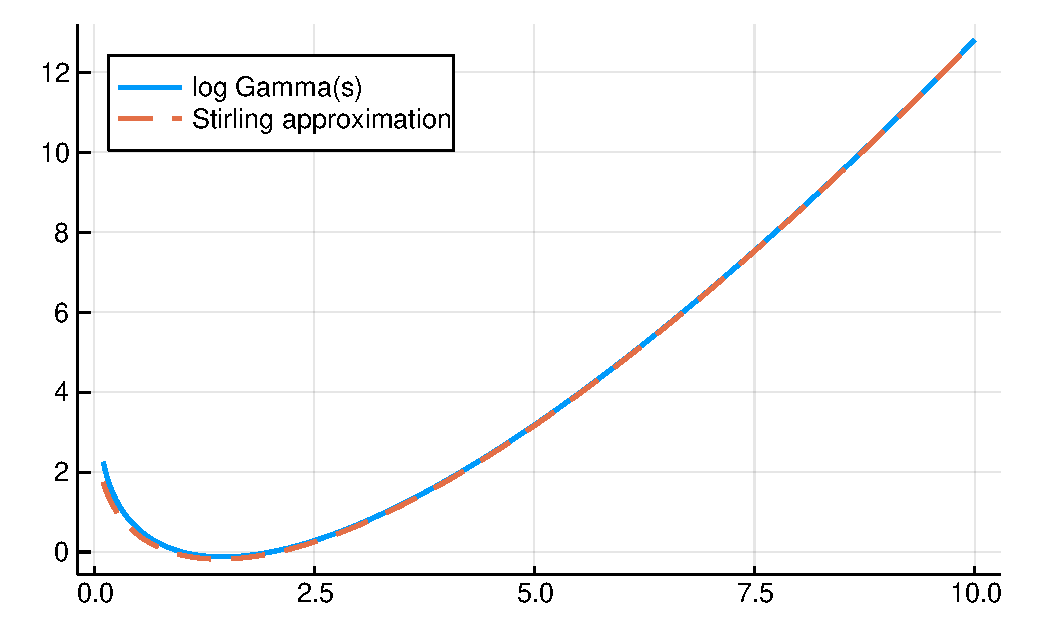
\includegraphics[width=0.8\linewidth]{figures/テスト_2_1.pdf}
\end{center}

\subsection{ガンマ分布とベータ分布の密度函数のグラフ}
\[
\theta,k,a,b>0
\]
に対して, ガンマ分布とベータ分布の確率密度函数がそれぞれ次のように定義される:
\[
\begin{aligned}
&
p(x) = \frac{1}{\theta^k \Gamma(k)} e^{-x/\theta} x^{k-1} \quad (x>0),
\\ &
q(x) = \frac{1}{B(a,b)} x^{a-1}(1-x)^{b-1} \quad (0 < x < 1).
\end{aligned}
\]
これらは $k,q,b$ が大きなとき, それぞれ正規分布の確率密度函数
\[
\begin{aligned}
f(x|\mu,\sigma^2) = \frac{1}{\sqrt{2\pi\sigma^2}}e^{-(x-\mu)^2/(2\sigma^2)}
\end{aligned}
\]
の $(\mu,\sigma^2)=(k\theta, k\theta^2), (a/(a+b), ab/((a+b)^2(a+b+1)))$ の場合でよく近似されるようになる(中心極限定理の特別な場合). そのことをグラフを描いて確認しよう.


\begin{lstlisting}
(*@\HLJLn{k}@*)(*@\HLJLp{,}@*) (*@\HLJLn{\ensuremath{\theta}}@*) (*@\HLJLoB{=}@*) (*@\HLJLni{100}@*)(*@\HLJLp{,}@*) (*@\HLJLni{1}@*)(*@\HLJLoB{/}@*)(*@\HLJLni{80}@*)
(*@\HLJLn{gdist}@*) (*@\HLJLoB{=}@*) (*@\HLJLnf{Gamma}@*)(*@\HLJLp{(}@*)(*@\HLJLn{k}@*)(*@\HLJLp{,}@*) (*@\HLJLn{\ensuremath{\theta}}@*)(*@\HLJLp{)}@*)
(*@\HLJLn{ndist}@*) (*@\HLJLoB{=}@*) (*@\HLJLnf{Normal}@*)(*@\HLJLp{(}@*)(*@\HLJLn{k}@*)(*@\HLJLoB{*}@*)(*@\HLJLn{\ensuremath{\theta}}@*)(*@\HLJLp{,}@*) (*@\HLJLoB{\ensuremath{\surd}}@*)(*@\HLJLn{k}@*)(*@\HLJLoB{*}@*)(*@\HLJLn{\ensuremath{\theta}}@*)(*@\HLJLp{)}@*)
(*@\HLJLn{x}@*) (*@\HLJLoB{=}@*) (*@\HLJLnf{range}@*)(*@\HLJLp{(}@*)(*@\HLJLni{0}@*)(*@\HLJLp{,}@*) (*@\HLJLnfB{2.7}@*)(*@\HLJLp{,}@*) (*@\HLJLn{length}@*)(*@\HLJLoB{=}@*)(*@\HLJLni{400}@*)(*@\HLJLp{)}@*)
(*@\HLJLnf{plot}@*)(*@\HLJLp{(}@*)(*@\HLJLn{size}@*)(*@\HLJLoB{=}@*)(*@\HLJLp{(}@*)(*@\HLJLni{500}@*)(*@\HLJLp{,}@*) (*@\HLJLni{300}@*)(*@\HLJLp{))}@*)
(*@\HLJLnf{title!}@*)(*@\HLJLp{(}@*)(*@\HLJLs{"Normal approximation of Gamma distribution"}@*)(*@\HLJLp{,}@*) (*@\HLJLn{titlefontsize}@*)(*@\HLJLoB{=}@*)(*@\HLJLni{12}@*)(*@\HLJLp{)}@*)
(*@\HLJLnf{plot!}@*)(*@\HLJLp{(}@*)(*@\HLJLn{legend}@*)(*@\HLJLoB{=:}@*)(*@\HLJLn{topright}@*)(*@\HLJLp{)}@*)
(*@\HLJLnf{plot!}@*)(*@\HLJLp{(}@*)(*@\HLJLn{x}@*)(*@\HLJLp{,}@*) (*@\HLJLn{pdf}@*)(*@\HLJLoB{.}@*)(*@\HLJLp{(}@*)(*@\HLJLn{gdist}@*)(*@\HLJLp{,}@*) (*@\HLJLn{x}@*)(*@\HLJLp{),}@*) (*@\HLJLn{label}@*)(*@\HLJLoB{=}@*)(*@\HLJLs{"Gamma(}@*)(*@\HLJLsi{{\$}k}@*)(*@\HLJLs{, }@*)(*@\HLJLsi{{\$}\ensuremath{\theta}}@*)(*@\HLJLs{)"}@*)(*@\HLJLp{,}@*) (*@\HLJLn{lw}@*)(*@\HLJLoB{=}@*)(*@\HLJLni{2}@*)(*@\HLJLp{)}@*)
(*@\HLJLnf{plot!}@*)(*@\HLJLp{(}@*)(*@\HLJLn{x}@*)(*@\HLJLp{,}@*) (*@\HLJLn{pdf}@*)(*@\HLJLoB{.}@*)(*@\HLJLp{(}@*)(*@\HLJLn{ndist}@*)(*@\HLJLp{,}@*) (*@\HLJLn{x}@*)(*@\HLJLp{),}@*) (*@\HLJLn{label}@*)(*@\HLJLoB{=}@*)(*@\HLJLs{"Normal approximation"}@*)(*@\HLJLp{,}@*) (*@\HLJLn{ls}@*)(*@\HLJLoB{=:}@*)(*@\HLJLn{dash}@*)(*@\HLJLp{,}@*) (*@\HLJLn{lw}@*)(*@\HLJLoB{=}@*)(*@\HLJLni{2}@*)(*@\HLJLp{)}@*)
\end{lstlisting}


\begin{center}
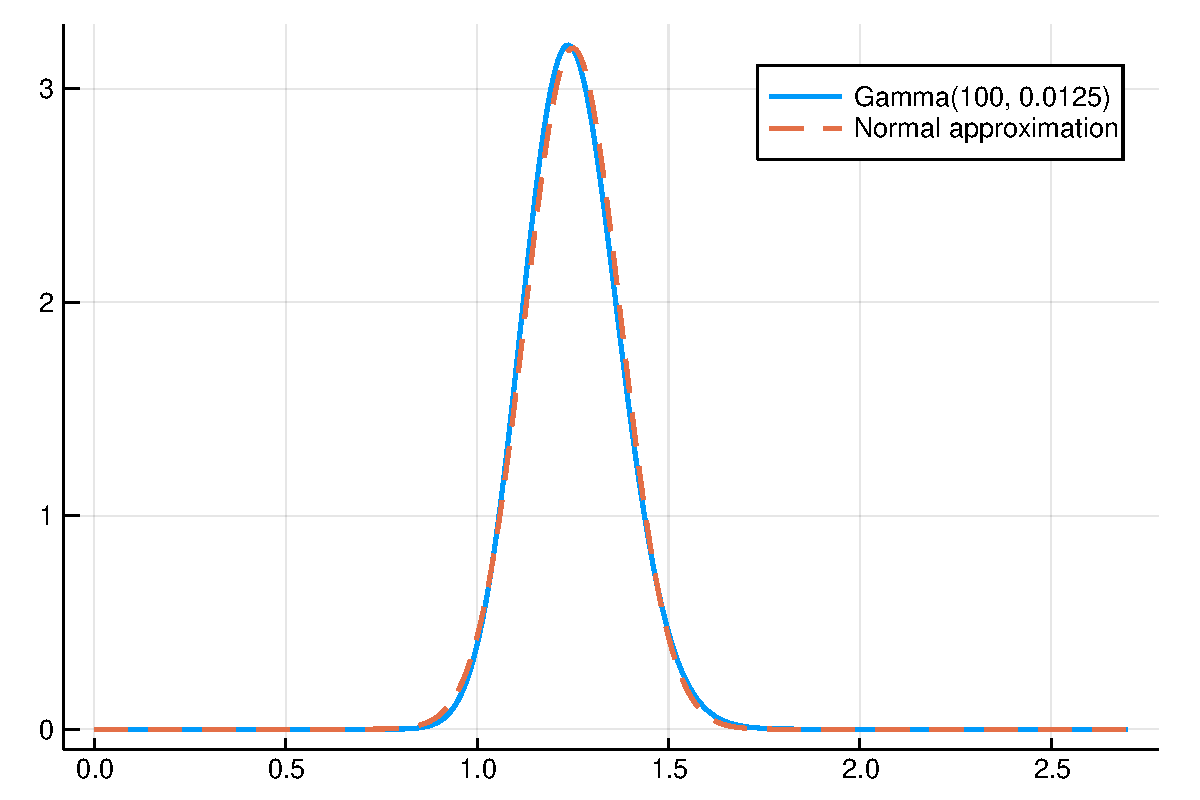
\includegraphics[width=0.8\linewidth]{figures/テスト_3_1.pdf}
\end{center}

\begin{lstlisting}
(*@\HLJLn{a}@*)(*@\HLJLp{,}@*) (*@\HLJLn{b}@*) (*@\HLJLoB{=}@*) (*@\HLJLni{40}@*)(*@\HLJLp{,}@*) (*@\HLJLni{60}@*)
(*@\HLJLn{bdist}@*) (*@\HLJLoB{=}@*) (*@\HLJLnf{Beta}@*)(*@\HLJLp{(}@*)(*@\HLJLn{a}@*)(*@\HLJLp{,}@*) (*@\HLJLn{b}@*)(*@\HLJLp{)}@*)
(*@\HLJLn{ndist}@*) (*@\HLJLoB{=}@*) (*@\HLJLnf{Normal}@*)(*@\HLJLp{(}@*)(*@\HLJLn{a}@*)(*@\HLJLoB{/}@*)(*@\HLJLp{(}@*)(*@\HLJLn{a}@*)(*@\HLJLoB{+}@*)(*@\HLJLn{b}@*)(*@\HLJLp{),}@*) (*@\HLJLoB{\ensuremath{\surd}}@*)(*@\HLJLp{(}@*)(*@\HLJLn{a}@*)(*@\HLJLoB{*}@*)(*@\HLJLn{b}@*)(*@\HLJLoB{/}@*)(*@\HLJLp{((}@*)(*@\HLJLn{a}@*)(*@\HLJLoB{+}@*)(*@\HLJLn{b}@*)(*@\HLJLp{)}@*)(*@\HLJLoB{{\textasciicircum}}@*)(*@\HLJLni{2}@*)(*@\HLJLoB{*}@*)(*@\HLJLp{(}@*)(*@\HLJLn{a}@*)(*@\HLJLoB{+}@*)(*@\HLJLn{b}@*)(*@\HLJLoB{+}@*)(*@\HLJLni{1}@*)(*@\HLJLp{))))}@*)
(*@\HLJLn{x}@*) (*@\HLJLoB{=}@*) (*@\HLJLnf{range}@*)(*@\HLJLp{(}@*)(*@\HLJLni{0}@*)(*@\HLJLp{,}@*) (*@\HLJLni{1}@*)(*@\HLJLp{,}@*) (*@\HLJLn{length}@*)(*@\HLJLoB{=}@*)(*@\HLJLni{400}@*)(*@\HLJLp{)}@*)
(*@\HLJLnf{plot}@*)(*@\HLJLp{(}@*)(*@\HLJLn{size}@*)(*@\HLJLoB{=}@*)(*@\HLJLp{(}@*)(*@\HLJLni{500}@*)(*@\HLJLp{,}@*) (*@\HLJLni{300}@*)(*@\HLJLp{))}@*)
(*@\HLJLnf{title!}@*)(*@\HLJLp{(}@*)(*@\HLJLs{"Normal approximation of Beta distribution"}@*)(*@\HLJLp{,}@*) (*@\HLJLn{titlefontsize}@*)(*@\HLJLoB{=}@*)(*@\HLJLni{12}@*)(*@\HLJLp{)}@*)
(*@\HLJLnf{plot!}@*)(*@\HLJLp{(}@*)(*@\HLJLn{legend}@*)(*@\HLJLoB{=:}@*)(*@\HLJLn{topright}@*)(*@\HLJLp{)}@*)
(*@\HLJLnf{plot!}@*)(*@\HLJLp{(}@*)(*@\HLJLn{x}@*)(*@\HLJLp{,}@*) (*@\HLJLn{pdf}@*)(*@\HLJLoB{.}@*)(*@\HLJLp{(}@*)(*@\HLJLn{bdist}@*)(*@\HLJLp{,}@*) (*@\HLJLn{x}@*)(*@\HLJLp{),}@*) (*@\HLJLn{label}@*)(*@\HLJLoB{=}@*)(*@\HLJLs{"Beta(}@*)(*@\HLJLsi{{\$}a}@*)(*@\HLJLs{, }@*)(*@\HLJLsi{{\$}b}@*)(*@\HLJLs{)"}@*)(*@\HLJLp{,}@*) (*@\HLJLn{lw}@*)(*@\HLJLoB{=}@*)(*@\HLJLni{2}@*)(*@\HLJLp{)}@*)
(*@\HLJLnf{plot!}@*)(*@\HLJLp{(}@*)(*@\HLJLn{x}@*)(*@\HLJLp{,}@*) (*@\HLJLn{pdf}@*)(*@\HLJLoB{.}@*)(*@\HLJLp{(}@*)(*@\HLJLn{ndist}@*)(*@\HLJLp{,}@*) (*@\HLJLn{x}@*)(*@\HLJLp{),}@*) (*@\HLJLn{label}@*)(*@\HLJLoB{=}@*)(*@\HLJLs{"Normal approximation"}@*)(*@\HLJLp{,}@*) (*@\HLJLn{ls}@*)(*@\HLJLoB{=:}@*)(*@\HLJLn{dash}@*)(*@\HLJLp{,}@*) (*@\HLJLn{lw}@*)(*@\HLJLoB{=}@*)(*@\HLJLni{2}@*)(*@\HLJLp{)}@*)
\end{lstlisting}


\begin{center}
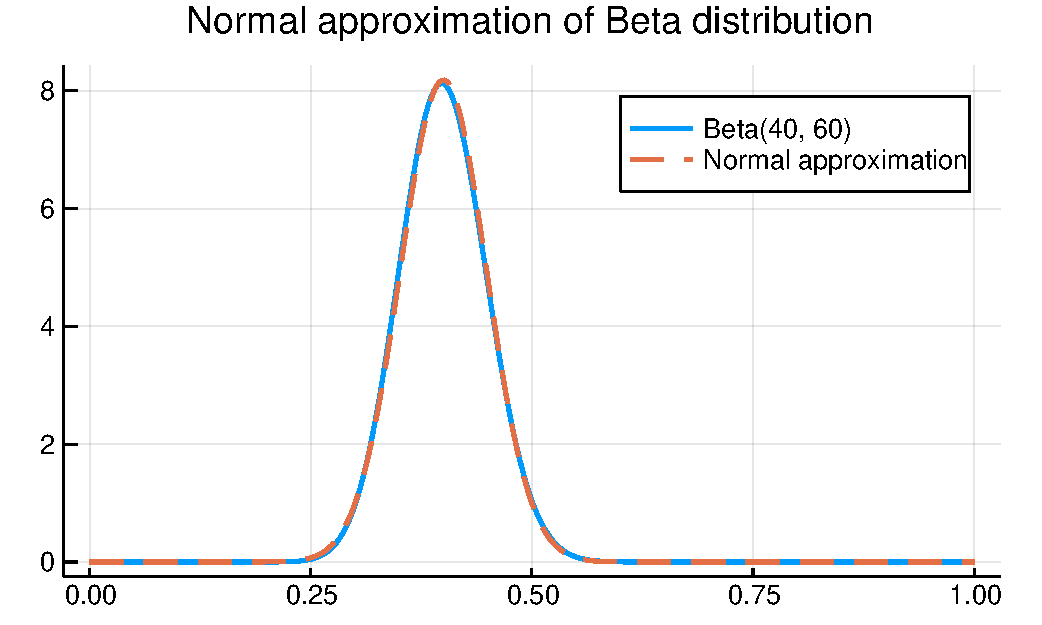
\includegraphics[width=0.8\linewidth]{figures/テスト_4_1.pdf}
\end{center}

\subsection{上で使ったガンマ函数の公式}
上で使ったガンマ分布の確率密度函数 $p(x)=e^{-x/\theta}x^{k-1}/(\theta^k\Gamma(k))$ ($x>0$) が確率密度函数であることを示すためには, それの $0$ から $\infty$ までの積分が $1$ になること, すなわち, 
\[
\int_0^\infty e^{-x/\theta} x^{k-1}\,dx = \theta^k \Gamma(k)
\quad (\theta, k > 0)
\]
が成立することを示さなければいけない. この公式は左辺を $x=\theta y$ で置換することによって得られる.

そのことはSymPyを使っても確かめられる. (注意: 以下の計算は\ensuremath{\theta}をSymPyの変数として使用しているので Python 2.7 では不可能. Python 3.x を使いましょう.)


\begin{lstlisting}
(*@\HLJLn{k}@*)(*@\HLJLp{,}@*) (*@\HLJLn{\ensuremath{\theta}}@*)(*@\HLJLp{,}@*) (*@\HLJLn{x}@*) (*@\HLJLoB{=}@*) (*@\HLJLnf{symbols}@*)(*@\HLJLp{(}@*)(*@\HLJLs{"k \ensuremath{\theta} x"}@*)(*@\HLJLp{,}@*) (*@\HLJLn{positive}@*)(*@\HLJLoB{=}@*)(*@\HLJLkc{true}@*)(*@\HLJLp{)}@*)
(*@\HLJLn{sol}@*) (*@\HLJLoB{=}@*) (*@\HLJLnf{simplify}@*)(*@\HLJLp{(}@*)(*@\HLJLnf{integrate}@*)(*@\HLJLp{(}@*)(*@\HLJLnf{exp}@*)(*@\HLJLp{(}@*)(*@\HLJLoB{-}@*)(*@\HLJLn{x}@*)(*@\HLJLoB{/}@*)(*@\HLJLn{\ensuremath{\theta}}@*)(*@\HLJLp{)}@*)(*@\HLJLoB{*}@*)(*@\HLJLn{x}@*)(*@\HLJLoB{{\textasciicircum}}@*)(*@\HLJLp{(}@*)(*@\HLJLn{k}@*)(*@\HLJLoB{-}@*)(*@\HLJLni{1}@*)(*@\HLJLp{),}@*) (*@\HLJLp{(}@*)(*@\HLJLn{x}@*)(*@\HLJLp{,}@*) (*@\HLJLni{0}@*)(*@\HLJLp{,}@*) (*@\HLJLn{oo}@*)(*@\HLJLp{)))}@*)
(*@\HLJLn{solstr}@*) (*@\HLJLoB{=}@*) (*@\HLJLnf{replace}@*)(*@\HLJLp{(}@*)(*@\HLJLn{sympy}@*)(*@\HLJLoB{.}@*)(*@\HLJLnf{latex}@*)(*@\HLJLp{(}@*)(*@\HLJLn{sol}@*)(*@\HLJLp{),}@*) (*@\HLJLs{"\ensuremath{\theta}"}@*)(*@\HLJLoB{=>}@*)(*@\HLJLs{"}@*)(*@\HLJLse{{\textbackslash}{\textbackslash}}@*)(*@\HLJLs{theta"}@*)(*@\HLJLp{)}@*)
(*@\HLJLnf{display}@*)(*@\HLJLp{(}@*)(*@\HLJLs{"text/html"}@*)(*@\HLJLp{,}@*) (*@\HLJLso{raw"{\$}{\$}{\textbackslash}int{\_}0{\textasciicircum}{\textbackslash}infty e{\textasciicircum}{\{}-x/{\textbackslash}theta{\}} x{\textasciicircum}{\{}k-1{\}}{\textbackslash},dx = "}@*) (*@\HLJLoB{*}@*) (*@\HLJLn{solstr}@*) (*@\HLJLoB{*}@*) (*@\HLJLso{raw"{\$}{\$}"}@*)(*@\HLJLp{);}@*)
\end{lstlisting}


$$\int_0^\infty e^{-x/\theta} x^{k-1}\,dx = \theta^{k} \Gamma\left(k\right)$$

\textbf{注意:} LaTeXStrings.jl の \texttt{latexstring()} を使用して同じ数式を表示させると, \texttt{weave(~, doctype="md2html")} でうまく数式が表示されなくなる. 上のように mimetype \texttt{text/html} で \texttt{display} を使用し, 行末に \texttt{;} を付ければうまく表示されるようになる.

\section{Riemannのゼータ函数}
Riemannのゼータ函数は $\real s > 1$ において
\[
\zeta(s) = \sum_{n=1}^\infty \frac{1}{n^s} \quad (\real s > 1)
\]
と定義され, 唯一の極 $s=1$ を除いた複素平面全体に解析接続される. 

Riemannのゼータ函数の $0\leqq \real s\leqq 1$ (critical strip)における零点を\textbf{非自明な零点}と呼ぶ. 

\textbf{Riemann予想:} Riemannのゼータ函数の非自明な零点はすべて直線 $\real s=1/2$ 上に乗っている. 

Riemannのゼータ函数の非自明な零点は素数の分布の精密な評価と関係している.

Riemann予想の成立を(数学的な証明にはならないが)数値的な計算で確認してみよう

\subsection{Riemannのゼータ函数の絶対値の対数のheatmap}

\begin{lstlisting}
(*@\HLJLnf{f}@*)(*@\HLJLp{(}@*)(*@\HLJLn{s}@*)(*@\HLJLp{)}@*) (*@\HLJLoB{=}@*) (*@\HLJLnf{max}@*)(*@\HLJLp{(}@*)(*@\HLJLnf{min}@*)(*@\HLJLp{(}@*)(*@\HLJLnf{log}@*)(*@\HLJLp{(}@*)(*@\HLJLnf{abs}@*)(*@\HLJLp{(}@*)(*@\HLJLnf{zeta}@*)(*@\HLJLp{(}@*)(*@\HLJLn{s}@*)(*@\HLJLp{))),}@*) (*@\HLJLni{3}@*)(*@\HLJLp{),}@*) (*@\HLJLoB{-}@*)(*@\HLJLni{5}@*)(*@\HLJLp{)}@*)
(*@\HLJLn{x}@*) (*@\HLJLoB{=}@*) (*@\HLJLnf{range}@*)(*@\HLJLp{(}@*)(*@\HLJLni{0}@*)(*@\HLJLp{,}@*) (*@\HLJLni{1}@*)(*@\HLJLp{,}@*) (*@\HLJLn{length}@*)(*@\HLJLoB{=}@*)(*@\HLJLni{100}@*)(*@\HLJLp{)}@*)
(*@\HLJLn{y}@*) (*@\HLJLoB{=}@*) (*@\HLJLnf{range}@*)(*@\HLJLp{(}@*)(*@\HLJLni{10}@*)(*@\HLJLp{,}@*) (*@\HLJLni{45}@*)(*@\HLJLp{,}@*) (*@\HLJLn{length}@*)(*@\HLJLoB{=}@*)(*@\HLJLni{400}@*)(*@\HLJLp{)}@*)
(*@\HLJLn{s}@*) (*@\HLJLoB{=}@*) @(*@\HLJLoB{.}@*) (*@\HLJLn{x}@*) (*@\HLJLoB{+}@*) (*@\HLJLn{im}@*)(*@\HLJLoB{*}@*)(*@\HLJLn{y}@*)(*@\HLJLoB{{\textquotesingle}}@*)
(*@\HLJLnf{plot}@*)(*@\HLJLp{(}@*)(*@\HLJLn{size}@*)(*@\HLJLoB{=}@*)(*@\HLJLp{(}@*)(*@\HLJLni{750}@*)(*@\HLJLp{,}@*) (*@\HLJLni{180}@*)(*@\HLJLp{))}@*)
(*@\HLJLnf{title!}@*)(*@\HLJLp{(}@*)(*@\HLJLs{"log(abs(zeta(x+iy)))"}@*)(*@\HLJLp{,}@*) (*@\HLJLn{titlefontsize}@*)(*@\HLJLoB{=}@*)(*@\HLJLni{12}@*)(*@\HLJLp{)}@*)
(*@\HLJLnf{heatmap!}@*)(*@\HLJLp{(}@*)(*@\HLJLn{y}@*)(*@\HLJLp{,}@*) (*@\HLJLn{x}@*)(*@\HLJLp{,}@*) (*@\HLJLn{f}@*)(*@\HLJLoB{.}@*)(*@\HLJLp{(}@*)(*@\HLJLn{s}@*)(*@\HLJLp{),}@*) (*@\HLJLn{color}@*)(*@\HLJLoB{=:}@*)(*@\HLJLn{thermal}@*)(*@\HLJLp{)}@*)
(*@\HLJLnf{xlabel!}@*)(*@\HLJLp{(}@*)(*@\HLJLs{"y"}@*)(*@\HLJLp{)}@*)
(*@\HLJLnf{ylabel!}@*)(*@\HLJLp{(}@*)(*@\HLJLs{"x"}@*)(*@\HLJLp{)}@*)
(*@\HLJLnf{hline!}@*)(*@\HLJLp{([}@*)(*@\HLJLnfB{0.5}@*)(*@\HLJLp{],}@*) (*@\HLJLn{ls}@*)(*@\HLJLoB{=:}@*)(*@\HLJLn{dot}@*)(*@\HLJLp{,}@*) (*@\HLJLn{color}@*)(*@\HLJLoB{=:}@*)(*@\HLJLn{cyan}@*)(*@\HLJLp{,}@*) (*@\HLJLn{label}@*)(*@\HLJLoB{=}@*)(*@\HLJLs{""}@*)(*@\HLJLp{)}@*)
\end{lstlisting}


\begin{center}
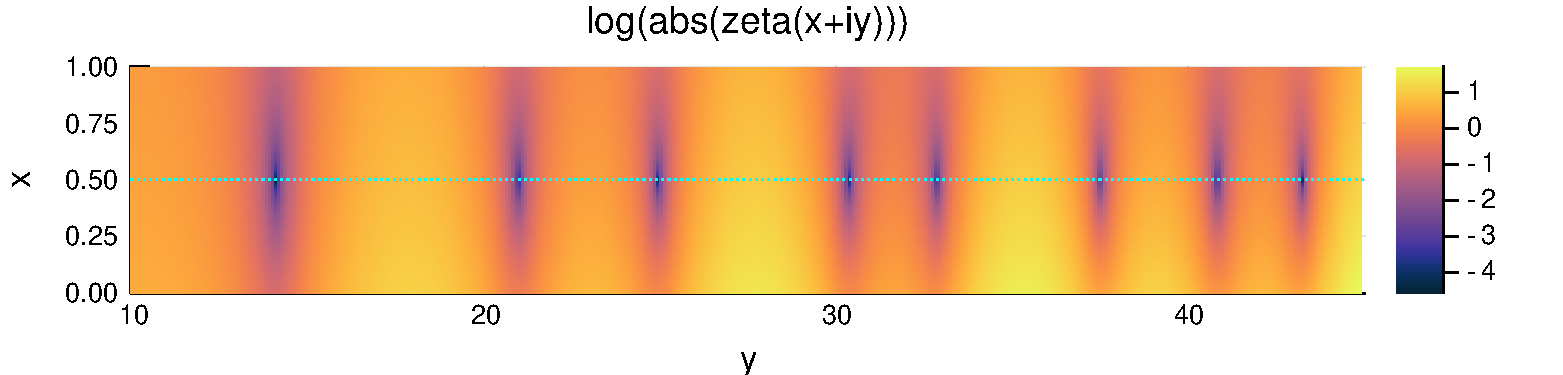
\includegraphics[width=0.8\linewidth]{figures/テスト_6_1.pdf}
\end{center}

\subsection{Riemannのゼータ函数の絶対値の Re s = 1/2 上の様子}

\begin{lstlisting}
(*@\HLJLnf{f}@*)(*@\HLJLp{(}@*)(*@\HLJLn{s}@*)(*@\HLJLp{)}@*) (*@\HLJLoB{=}@*) (*@\HLJLnf{abs}@*)(*@\HLJLp{(}@*)(*@\HLJLnf{zeta}@*)(*@\HLJLp{(}@*)(*@\HLJLn{s}@*)(*@\HLJLp{))}@*)
(*@\HLJLn{x}@*) (*@\HLJLoB{=}@*) (*@\HLJLni{1}@*)(*@\HLJLoB{/}@*)(*@\HLJLni{2}@*)
(*@\HLJLn{y}@*) (*@\HLJLoB{=}@*) (*@\HLJLnf{range}@*)(*@\HLJLp{(}@*)(*@\HLJLni{10}@*)(*@\HLJLp{,}@*) (*@\HLJLni{45}@*)(*@\HLJLp{,}@*) (*@\HLJLn{length}@*)(*@\HLJLoB{=}@*)(*@\HLJLni{1000}@*)(*@\HLJLp{)}@*)
(*@\HLJLn{s}@*) (*@\HLJLoB{=}@*) @(*@\HLJLoB{.}@*) (*@\HLJLn{x}@*) (*@\HLJLoB{+}@*) (*@\HLJLn{im}@*)(*@\HLJLoB{*}@*)(*@\HLJLn{y}@*)
(*@\HLJLnf{plot}@*)(*@\HLJLp{(}@*)(*@\HLJLn{size}@*)(*@\HLJLoB{=}@*)(*@\HLJLp{(}@*)(*@\HLJLni{720}@*)(*@\HLJLp{,}@*) (*@\HLJLni{200}@*)(*@\HLJLp{))}@*)
(*@\HLJLnf{title!}@*)(*@\HLJLp{(}@*)(*@\HLJLs{"abs(zeta(0.5+iy)))"}@*)(*@\HLJLp{,}@*) (*@\HLJLn{titlefontsize}@*)(*@\HLJLoB{=}@*)(*@\HLJLni{12}@*)(*@\HLJLp{)}@*)
(*@\HLJLnf{plot!}@*)(*@\HLJLp{(}@*)(*@\HLJLn{y}@*)(*@\HLJLp{,}@*) (*@\HLJLn{f}@*)(*@\HLJLoB{.}@*)(*@\HLJLp{(}@*)(*@\HLJLn{s}@*)(*@\HLJLp{),}@*) (*@\HLJLn{label}@*)(*@\HLJLoB{=}@*)(*@\HLJLs{""}@*)(*@\HLJLp{)}@*)
(*@\HLJLnf{xlabel!}@*)(*@\HLJLp{(}@*)(*@\HLJLs{"y"}@*)(*@\HLJLp{)}@*)
\end{lstlisting}


\begin{center}
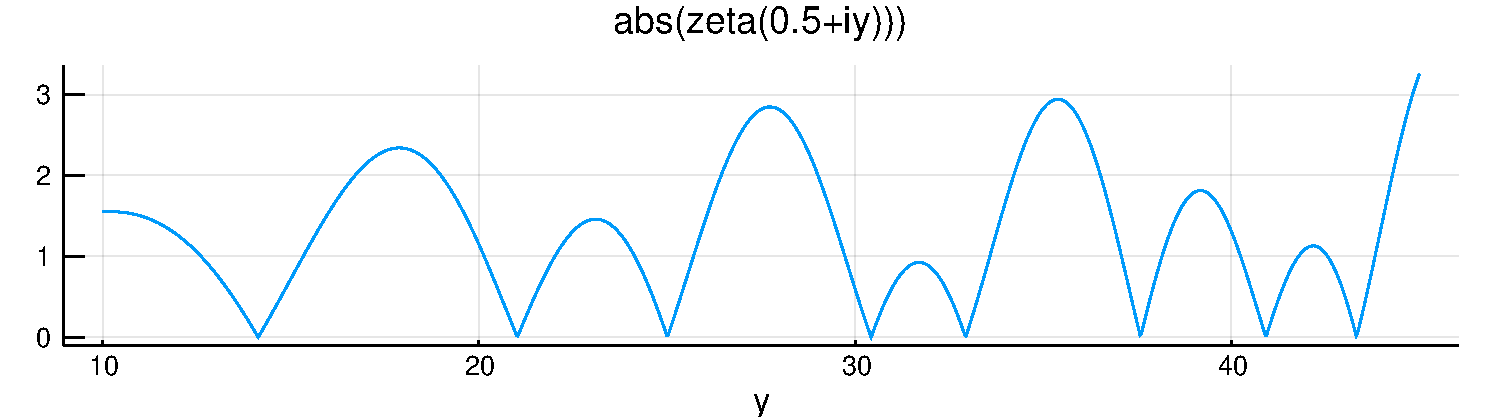
\includegraphics[width=0.8\linewidth]{figures/テスト_7_1.pdf}
\end{center}

\subsection{Riemannのゼータ函数の Re s = 1/2 上での複素数値}
直線 $\real s = 1/2$ での $\zeta(s)$ の値は何度も繰り返し複素平面の原点 $0$ を通る.


\begin{lstlisting}
(*@\HLJLn{x}@*) (*@\HLJLoB{=}@*) (*@\HLJLni{1}@*)(*@\HLJLoB{/}@*)(*@\HLJLni{2}@*)
(*@\HLJLn{y}@*) (*@\HLJLoB{=}@*) (*@\HLJLnf{range}@*)(*@\HLJLp{(}@*)(*@\HLJLni{0}@*)(*@\HLJLp{,}@*) (*@\HLJLni{45}@*)(*@\HLJLp{,}@*) (*@\HLJLn{length}@*)(*@\HLJLoB{=}@*)(*@\HLJLni{1000}@*)(*@\HLJLp{)}@*)
(*@\HLJLn{s}@*) (*@\HLJLoB{=}@*) @(*@\HLJLoB{.}@*) (*@\HLJLn{x}@*) (*@\HLJLoB{+}@*) (*@\HLJLn{im}@*)(*@\HLJLoB{*}@*)(*@\HLJLn{y}@*)
(*@\HLJLn{w}@*) (*@\HLJLoB{=}@*) (*@\HLJLn{zeta}@*)(*@\HLJLoB{.}@*)(*@\HLJLp{(}@*)(*@\HLJLn{s}@*)(*@\HLJLp{)}@*)
(*@\HLJLnf{plot}@*)(*@\HLJLp{(}@*)(*@\HLJLn{size}@*)(*@\HLJLoB{=}@*)(*@\HLJLp{(}@*)(*@\HLJLni{500}@*)(*@\HLJLp{,}@*)(*@\HLJLni{400}@*)(*@\HLJLp{),}@*) (*@\HLJLn{legend}@*)(*@\HLJLoB{=:}@*)(*@\HLJLn{topleft}@*)(*@\HLJLp{)}@*)
(*@\HLJLnf{title!}@*)(*@\HLJLp{(}@*)(*@\HLJLs{"zeta(0.5+it) for 0 < t < 45"}@*)(*@\HLJLp{,}@*) (*@\HLJLn{titlefontsize}@*)(*@\HLJLoB{=}@*)(*@\HLJLni{12}@*)(*@\HLJLp{)}@*)
(*@\HLJLnf{plot!}@*)(*@\HLJLp{(}@*)(*@\HLJLnf{real}@*)(*@\HLJLp{(}@*)(*@\HLJLn{w}@*)(*@\HLJLp{),}@*) (*@\HLJLnf{imag}@*)(*@\HLJLp{(}@*)(*@\HLJLn{w}@*)(*@\HLJLp{),}@*) (*@\HLJLn{label}@*)(*@\HLJLoB{=}@*)(*@\HLJLs{"zeta(0.5+it)"}@*)(*@\HLJLp{)}@*)
(*@\HLJLnf{scatter!}@*)(*@\HLJLp{([}@*)(*@\HLJLni{0}@*)(*@\HLJLp{],}@*) (*@\HLJLp{[}@*)(*@\HLJLni{0}@*)(*@\HLJLp{],}@*) (*@\HLJLn{markersize}@*)(*@\HLJLoB{=}@*)(*@\HLJLni{2}@*)(*@\HLJLp{,}@*) (*@\HLJLn{label}@*)(*@\HLJLoB{=}@*)(*@\HLJLs{""}@*)(*@\HLJLp{)}@*)
(*@\HLJLnf{xlabel!}@*)(*@\HLJLp{(}@*)(*@\HLJLs{"x"}@*)(*@\HLJLp{)}@*)
(*@\HLJLnf{ylabel!}@*)(*@\HLJLp{(}@*)(*@\HLJLs{"y"}@*)(*@\HLJLp{)}@*)
(*@\HLJLnf{annotate!}@*)(*@\HLJLp{([(}@*)(*@\HLJLoB{-}@*)(*@\HLJLnfB{1.25}@*)(*@\HLJLp{,}@*) (*@\HLJLnfB{0.1}@*)(*@\HLJLp{,}@*) (*@\HLJLs{"zeta(0.5)"}@*)(*@\HLJLp{,}@*) (*@\HLJLni{9}@*)(*@\HLJLp{)])}@*)
(*@\HLJLnf{annotate!}@*)(*@\HLJLp{([(}@*)(*@\HLJLnfB{2.55}@*)(*@\HLJLp{,}@*) (*@\HLJLnfB{1.7}@*)(*@\HLJLp{,}@*) (*@\HLJLs{"zeta(0.5+45i)"}@*)(*@\HLJLp{,}@*) (*@\HLJLni{9}@*)(*@\HLJLp{)])}@*)
\end{lstlisting}


\begin{center}
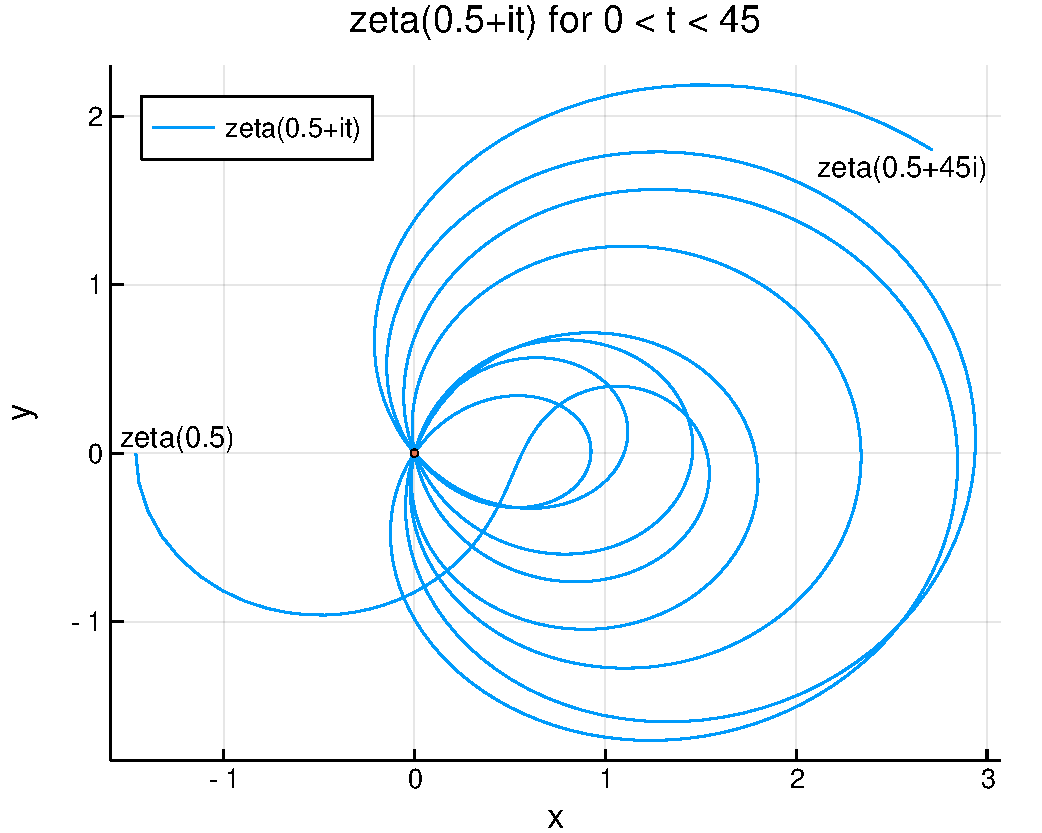
\includegraphics[width=0.8\linewidth]{figures/テスト_8_1.pdf}
\end{center}

\subsection{Riemannのゼータ函数の Re s = 0.6 上での複素数値}
直線 $\real s = 0.6$ での $\zeta(s)$ の値を計算すると複素平面の原点を避けて通っていることがわかる.


\begin{lstlisting}
(*@\HLJLn{x}@*) (*@\HLJLoB{=}@*) (*@\HLJLnfB{0.6}@*)
(*@\HLJLn{y}@*) (*@\HLJLoB{=}@*) (*@\HLJLnf{range}@*)(*@\HLJLp{(}@*)(*@\HLJLni{0}@*)(*@\HLJLp{,}@*) (*@\HLJLni{45}@*)(*@\HLJLp{,}@*) (*@\HLJLn{length}@*)(*@\HLJLoB{=}@*)(*@\HLJLni{1000}@*)(*@\HLJLp{)}@*)
(*@\HLJLn{s}@*) (*@\HLJLoB{=}@*) @(*@\HLJLoB{.}@*) (*@\HLJLn{x}@*) (*@\HLJLoB{+}@*) (*@\HLJLn{im}@*)(*@\HLJLoB{*}@*)(*@\HLJLn{y}@*)
(*@\HLJLn{w}@*) (*@\HLJLoB{=}@*) (*@\HLJLn{zeta}@*)(*@\HLJLoB{.}@*)(*@\HLJLp{(}@*)(*@\HLJLn{s}@*)(*@\HLJLp{)}@*)
(*@\HLJLnf{plot}@*)(*@\HLJLp{(}@*)(*@\HLJLn{size}@*)(*@\HLJLoB{=}@*)(*@\HLJLp{(}@*)(*@\HLJLni{500}@*)(*@\HLJLp{,}@*)(*@\HLJLni{400}@*)(*@\HLJLp{),}@*) (*@\HLJLn{legend}@*)(*@\HLJLoB{=:}@*)(*@\HLJLn{topleft}@*)(*@\HLJLp{)}@*)
(*@\HLJLnf{title!}@*)(*@\HLJLp{(}@*)(*@\HLJLs{"zeta(0.6+it) for 0 < t < 45"}@*)(*@\HLJLp{,}@*) (*@\HLJLn{titlefontsize}@*)(*@\HLJLoB{=}@*)(*@\HLJLni{12}@*)(*@\HLJLp{)}@*)
(*@\HLJLnf{plot!}@*)(*@\HLJLp{(}@*)(*@\HLJLnf{real}@*)(*@\HLJLp{(}@*)(*@\HLJLn{w}@*)(*@\HLJLp{),}@*) (*@\HLJLnf{imag}@*)(*@\HLJLp{(}@*)(*@\HLJLn{w}@*)(*@\HLJLp{),}@*) (*@\HLJLn{label}@*)(*@\HLJLoB{=}@*)(*@\HLJLs{"zeta(0.6+it)"}@*)(*@\HLJLp{)}@*)
(*@\HLJLnf{scatter!}@*)(*@\HLJLp{([}@*)(*@\HLJLni{0}@*)(*@\HLJLp{],}@*) (*@\HLJLp{[}@*)(*@\HLJLni{0}@*)(*@\HLJLp{],}@*) (*@\HLJLn{markersize}@*)(*@\HLJLoB{=}@*)(*@\HLJLni{2}@*)(*@\HLJLp{,}@*) (*@\HLJLn{label}@*)(*@\HLJLoB{=}@*)(*@\HLJLs{""}@*)(*@\HLJLp{)}@*)
(*@\HLJLnf{xlabel!}@*)(*@\HLJLp{(}@*)(*@\HLJLs{"x"}@*)(*@\HLJLp{)}@*)
(*@\HLJLnf{ylabel!}@*)(*@\HLJLp{(}@*)(*@\HLJLs{"y"}@*)(*@\HLJLp{)}@*)
(*@\HLJLnf{annotate!}@*)(*@\HLJLp{([(}@*)(*@\HLJLoB{-}@*)(*@\HLJLnfB{1.6}@*)(*@\HLJLp{,}@*) (*@\HLJLnfB{0.1}@*)(*@\HLJLp{,}@*) (*@\HLJLs{"zeta(0.6)"}@*)(*@\HLJLp{,}@*) (*@\HLJLni{9}@*)(*@\HLJLp{)])}@*)
(*@\HLJLnf{annotate!}@*)(*@\HLJLp{([(}@*)(*@\HLJLnfB{2.55}@*)(*@\HLJLp{,}@*) (*@\HLJLnfB{1.4}@*)(*@\HLJLp{,}@*) (*@\HLJLs{"zeta(0.6+45i)"}@*)(*@\HLJLp{,}@*) (*@\HLJLni{9}@*)(*@\HLJLp{)])}@*)
\end{lstlisting}


\begin{center}
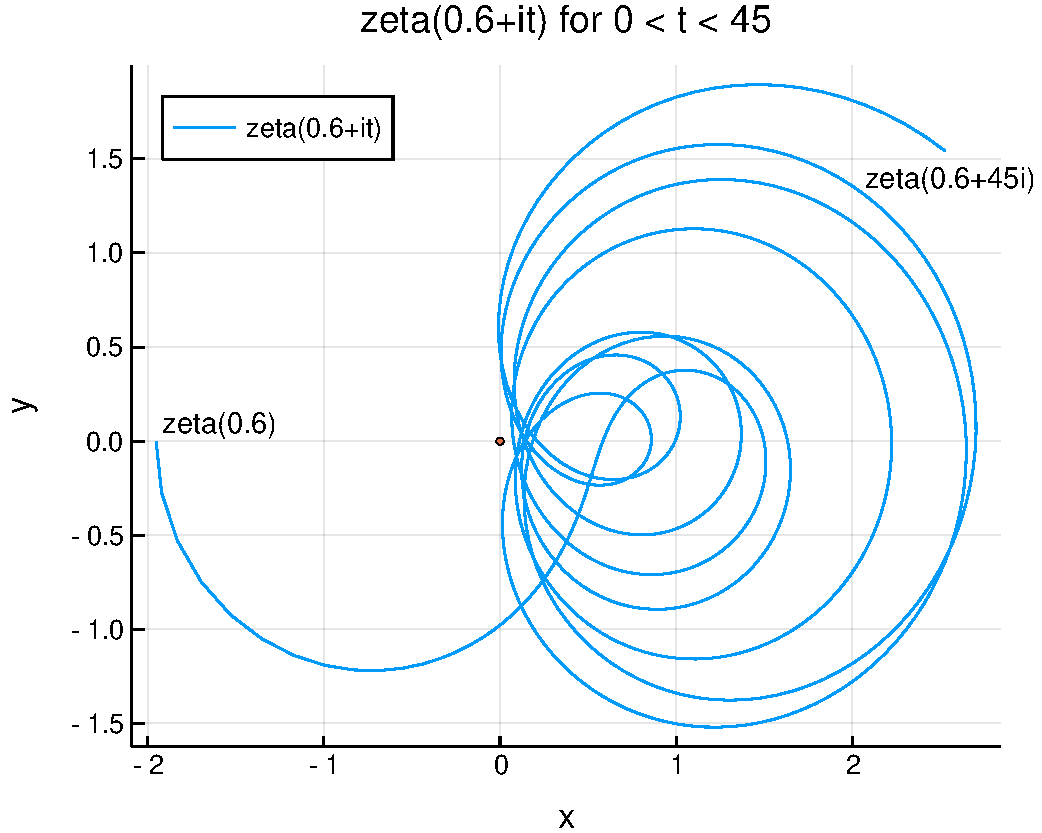
\includegraphics[width=0.8\linewidth]{figures/テスト_9_1.pdf}
\end{center}

\section{手書きのノート}
\subsection{ガンマ函数とベータ函数入門(1)}
\begin{center}
\includegraphics[width=0.8\linewidth]{images/GammaBeta01.jpg}
\end{center}


\subsection{ガンマ函数とベータ函数入門(2)}
\begin{center}
\includegraphics[width=0.8\linewidth]{images/GammaBeta02.jpg}
\end{center}


\subsection{Hurwitzのゼータ函数とガンマ函数の関係}
\begin{center}
\includegraphics[width=0.8\linewidth]{images/HurwitzGamma.jpg}
\end{center}




\end{document}
